\documentclass{article}

\usepackage{graphicx}
\usepackage{graphpap}


\usepackage{fancyhdr}



%%%%%%%%%%%%%%%%%%%%%%%%%%%%%%%%%%%%%%%%5
%
%  Set Up Margins

%%%%%%%%%%%%%%%%%%%%%%%%%%%%%%%%%%%%%%%%%%%%%%%%%
% include file for:
%      Critical Page setup dimensions
%            DO NOT MODIFY
%       (for help see "Latex Line by Line" p 260)
%
\setlength\oddsidemargin{0in}
\setlength\evensidemargin{0in}

\usepackage[left=0.98in, right=0.98in, top=1.0in, bottom=1.0in]{geometry}

% %Top Margin and header
% \setlength\voffset{-0.94in}
% \setlength\topmargin{0.25in}
% \setlength\headheight{0.25in}
% %\setlength\headwidth{6.5in}
% \setlength\headsep{0.25in}
% %Body
% \setlength\textwidth{6.5in}
% \setlength\textheight{9.50in}
% %Footer
% %\setlength\footheight{0.5in}
% \setlength\footskip{0.3750in}
% Line spacing for 6 lines per inch
\linespread{0.894}  % 1.0 = single    1.6 = double
%
%          END of Critical Page Setup Dimensions
%%%%%%%%%%%%%%%%%%%%%%%%%%%%%%%%%%%%%%%%%%%%%%%%%%%

%%%%%%%%%%%%%%%%%%%%%%%%%%%%%%%%%%%%%%%%%%%%%%%%%%%
%
% Useful style and math macros
%


\newcommand\Dfrac[2]{\frac{\displaystyle #1}{\displaystyle #2}}
\newcommand\beq{\begin{equation}}
\newcommand\eeq{\end{equation}}

\newcommand\bmat{\begin{bmatrix}}
\newcommand\emat{\end{bmatrix}}

\newenvironment{solution}
{\vspace{0.125in} {\bf SOLUTION:} \\ }
{\vspace{0.25in}}



%%%%%%%%%%%%%%%%%%%%%%%%%%%%%%%%%%%%%%%%%%%%%%%%%
%
%         Page format Mods HERE
%
%Mod's to page size for this document
\addtolength\textwidth{0cm}
\addtolength\oddsidemargin{0cm}
\addtolength\headsep{0cm}
\addtolength\textheight{0cm}
%\linespread{0.894}   % 0.894 = 6 lines per inch, 1 = "single",  1.6 = "double"

%%%%%%%%%%%%%%%%%%%%%%%%%%%%% HEADER / FOOTER
\pagestyle{fancy}
%%%%%  Page header/footer fields for "NSF Style" proposal
%%%%%  \chead will be changed with each section
\lhead{\small\sc EE543}
\rhead{}
\chead{Scilab Programming Assignments}
\lfoot{Hannaford, U. of Washington}
\rfoot{\today}
\cfoot{\thepage}
%\renewcommand\headrulewidth{1pt}
%\renewcommand\footrulewidth{1pt}

\begin{document}

%%%%%%%%%%%%%%%%%%%%%%%%%%%%%%%%%%%%%%%%%%%%%%%%%%%%%%
%%%%** Section 1
\section{Rotations I}

We need a few easy functions to rapidly generate rotation matrices.  {\bf We will represent all angles in degrees.}

You may do these assignments in Matlab if you prefer. 
%%%%** Section 1.1
\subsection{Functions}
Write the following *lab functions:

\begin{itemize}
  \item {\tt R = rotx(theta)}  Produce a 3x3 rotation matrix about the $x$ axis by $\theta$ degrees.
  \item {\tt R = roty(theta)}  Produce a 3x3 rotation matrix about the $y$ axis by $\theta$ degrees.
  \item {\tt R = rotz(theta)}  Produce a 3x3 rotation matrix about the $z$ axis by $\theta$ degrees.
  \item {\tt R = rrpy(r,p,y)}  Produce a 3x3 rotation matrix to represent roll, pitch, and yaw rotations by $r, p, y$ respectively.
\end{itemize}

%%%%** Section 1.2
\subsection{Test Cases}
Repeat the computations below and compare your results.

\begin{verbatim}

// compute product of some rotations

A = rotx(30) * roty(60) * rotz(17.5)

-->A
 A  =

    0.4768585  - 0.1503529    0.8660254
    0.6733904    0.6957337  - 0.25
  - 0.5649348    0.7023878    0.4330127


// compute roll pitch yaw matrix two ways:
B = rotz(30) * roty(40) * rotx(50);
C = rrpy(50,40,30)

-->B-C
 ans  =

    0.    0.    0.
    0.    0.    0.
    0.    0.    0.


\end{verbatim}


\newpage
%%%%%%%%%%%%%%%%%%%%%%%%%%%%%%%%%%%%%%%%%%%%%%%%%%%%%%
%%%%** Section 2
\section{Rotations II and Homogeneous Transformations}

In this exercise we will create more advanced rotation matrix functions.

%%%%** Section 2.1
\subsection{Functions}
Write the following *lab functions:

\begin{itemize}
  \item {\tt R = equiv(K, theta)}  	Compute the rotation matrix corresponding to rotation by $\theta$ about an axis $K$ represented by a 3-vector.
  \item {\tt q = quaternion(K, theta)}  Compute the unit quaternion corresponding to rotation by $\theta$ about an axis $K$ represented by a 3-vector.
  \item {\tt q = qcomp(q1)} 		Compute the quaternion complement of any quaterion, $q1$.
  \item {\tt q1 = qtimes(q2,q3)} 	Compute the product of two quaterions $q2,q3$.
  \item {\tt T = trans4(v,r) }		Compute a 4x4 Homogeneous transform which represents translation by distance $r$ in a direction $v$ (v is a 3-vector).
  \item {\tt T = rot4(R)}               Generate a 4x4 version of rotation matrix {\tt R}.
\end{itemize}



%%%%** Section 2.2
\subsection{Test Cases}

\begin{verbatim}

-->K=[0 1 0 ]'
 K  =

    0.
    1.
    0.

-->equiv(K,45)
 ans  =

    0.7071068    0.    0.7071068
    0.           1.    0.
  - 0.7071068    0.    0.7071068


K = [1 2 3]';
R = equiv(K, 45);

-->R
 R  =

    0.7280277  - 0.5251048    0.4407273
    0.6087886    0.7907906  - 0.0634566
  - 0.3152016    0.3145079    0.8953953


-->// Quaternion

-->q1 = quaternion(K, 45);
-->q2 = qcomp(q1);
-->q3 = qtimes(q1,q2);
 -->K
 K  =

    1.
    2.
    3.

-->q1
 q1  =

    0.9238795
    0.1022764
    0.2045529
    0.3068293

-->q2
 q2  =

    0.9238795
  - 0.1022764
  - 0.2045529
  - 0.3068293

-->q3
 q3  =

    1.
    0.
    6.939D-18
    0.



//   2. Homogeneous Transforms

-->T1 = trans4(K, 10);
-->T2 = rot4(roty(45));
-->T1
 T1  =

    1.    0.    0.    2.6726124
    0.    1.    0.    5.3452248
    0.    0.    1.    8.0178373
    0.    0.    0.    1.

-->T2
 T2  =

    0.7071068    0.    0.7071068    0.
    0.           1.    0.           0.
  - 0.7071068    0.    0.7071068    0.
    0.           0.    0.           1.

-->T3=T1*T2
 T3  =

    0.7071068    0.    0.7071068    2.6726124
    0.           1.    0.           5.3452248
  - 0.7071068    0.    0.7071068    8.0178373
    0.           0.    0.           1.
\end{verbatim}





\newpage
%%%%%%%%%%%%%%%%%%%%%%%%%%%%%%%%%%%%%%%%%%%%%%%%%%%%%%
%%%%** Section 3
\section{Forward Kinematics}



%%%%** Section 3.1
\subsection{Functions}
Write the following *lab functions:

\begin{itemize}
  \item {\tt T = link(aln1,an1,dn,thn) }	Compute the 4x4 link transform matrix as a function of the four DH parameters for that link.
  \item {\tt T = hinv(T1)}			Compute the inverse of homogeneous transform, $T1$, in closed form.
\end{itemize}



%%%%** Section 3.2
\subsection{Test Cases}

Let's compute the position and orientation of frame 6 for the following DH table

\vspace{0.1in}
\begin{tabular}{|c|c|c|c|} \hline
$\alpha_{N-1}$	& $a_{N-1}$ 	& $d_N$	&	$\theta_N$	\\ \hline
0		& 0		& 0	& 	$\theta_1$	\\ \hline
90		& 0		& 0	& 	$\theta_2$	\\ \hline
-90		& 0.37		& 0	&	$\theta_3$	\\ \hline
90		& 0.5		& 0.25	&       $\theta_4$	\\ \hline
0		& 0.1		& 0.0	& 	$\theta_5$	\\ \hline
\end{tabular}
\vspace{0.1in}

Where $\theta_1=0^\circ,\; \theta_2=30^\circ\; \theta_3=45^\circ, \; \theta_4 = 37^\circ,\; \theta_5=32^\circ$.

\begin{verbatim}



-->th1= 0; th2=30;th3=45;th4=37;th5=32;

-->

-->T01 = link(0,     0,  0, th1);

-->T12 = link(90,    0,  0, th2);

-->T23 = link(-90, .37,  0, th3);

-->T34 = link(90,  0.5,.25, th4);

-->T45 = link(0,    .1,  0, th5);

-->

-->T05 = T01*T12*T23*T45
 T05  =

    0.9893499  - 0.1355545  - 0.0530268    0.4690227
    0.1357455    0.9907437  - 8.615D-20    0.0079494
    0.0525359  - 0.0071981    0.9985931    0.0249058
    0.           0.           0.           1.


\end{verbatim}

\newpage
%%%%%%%%%%%%%%%%%%%%%%%%%%%%%%%%%%%%%%%%%%%%%%%%%%%%%%
%%%%** Section 4
\section{Velocity Propagation}


%%%%** Section 4.1
\subsection{Functions}

Write the following *lab functions:

\begin{itemize}
  \item {\tt Np1wNp1 = wprop(TNNp1, NwN, thetadot)}		Compute the angular velocity propagation from link N to N+1. ({\tt NwN} = ${^N\omega_N}$, {\tt TNNp1} = ${^N_{N+1}T}$).
  \item {\tt Np1VNp1 = vprop(TNNp1, NwN, NVN, ddot)}		Compute the linear  velocity propagation from link N to N+1. ({\tt NVN} = ${^NV_N}$, {\tt ddot} = $\dot{d}_N$).
\end{itemize}




%%%%** Section 4.2
\subsection{Test Cases}

\begin{verbatim}
//  *lab assignment 4: velocity propagation
//   test cases

exec('kinfunc.sce',-1);
// All DH parameters

al0 = 0;    al1 = -90;    al2 = 180;    al3 = 90;
a0 = 0;     a1 = 1;      a2 = 0;      a3 = 2;
d1 = 3;     d2 = 1.5;    d3 = 1;      d4 = 0;

//Pose
th1 = 90;   th2 = 0;     th3 = 45;    th4 = 137;

// Joint velocities
// (only one of each pair should be non-zero)
dd1 =    0;  // m/sec
thd1 =  20;  // deg/sec
dd2 =    0.7;
thd2 =   0;
dd3  =   0;
thd3 =  10;
dd4  =   0;
thd4 = -16;

//  The link transforms
T01 = link(al0,a0,d1,th1);
T12 = link(al1,a1,d2,th2);
T23 = link(al2,a2,d3,th3);
T34 = link(al3,a3,d4,th4);

w00 = [0,0,0]';  // base is not moving
v00 = [0,0,0]';

//angular velocity propagation
w11 = wprop(T01,w00,thd1);
w22 = wprop(T12,w11,thd2);
w33 = wprop(T23,w22,thd3);
w44 = wprop(T34,w33,thd4);

// linear velocity propagation
v11 = vprop(T01,w00,v00,dd1);
v22 = vprop(T12,w11,v11,dd2);
v33 = vprop(T23,w22,v22,dd3);
v44 = vprop(T34,w33,v33,dd4);

// printf("Velocities: w44: %6.2f  \n",w44);
printf("Velocities: w44: %6.2f    v44: %6.2f\n",w44,v44);

-->exec('/home/blake/Dropbox/543/543instructor/Scilab/vproptestcase.sce', -1)
Velocities: w44:  -3.52    v44: -28.24
Velocities: w44: -16.96    v44:  40.65
Velocities: w44: -30.14    v44: -27.07
\end{verbatim}


\newpage
%%%%%%%%%%%%%%%%%%%%%%%%%%%%%%%%%%%%%%%%%%%%%%%%%%%%%%
%%%%** Section 5
\section{Gravity Compensation and Trajectory Generation}


%%%%** Section 5.1
\subsection{Functions}


Write the following *lab functions:

\begin{itemize}
  \item {\tt a = polyparams(thA, thB, dt)}   Compute the coefficients of the third order polynomial trajectory (see section 7.3.1)
  \item {\tt [acc,VM,tacc] = lin\_parab\_init(thA, thB, dt) }   Compute parameters for linear trajectories with parabolic blends. (see example 7.2)
  \item {\tt theta = lin\_parab\_run(t, t\_0, thA, thB, dt,  acc, VM, tacc)} Compute the linear/parabolic trajectory at each point in time.  (also see example 7.2)
  \item {\tt T = tcat(T1,T2) } Combine 4x4 T-matrices into a 3 dimensional matrix (this way we can step through the links of a manipulator in a loop). After this step, T(:,:,1) = T1, T(:,:,2) = T2.
  \item {\tt t = jtorque(T,C,M,g); } Compute torque on joint i based on centers of mass, masses, and T-matrices. Where
  \begin{itemize}
      \item T = 3dim matrix of Tmatrices (generated by tcat)
      \item C = array of COMvectors (Cii)
      \item M = array of masses (Mi)
      \item g = gravity vector in frame 0
      \item number of links = length(M)
  \end{itemize}
\end{itemize}


\subsection{Test Cases}
\begin{verbatim}

//testcase:  trajectory generation and dynamics
// Trajectory Generation Test cases
//   Scilab programming assignment 5

clear all;

exec("tg_gravcomp.sce",-1);

/////////////////////////////
//  3rd order polynomial traj:
//      ThA = 20,  ThB = 60
//      Dt = 0.45 sec

a= polyparams(20, 60, 0.45);

t = 0:0.02:0.45;

y_poly = a(1) + a(2)*t + a(3)*t.*t + a(4)*t.*t.*t;


/////////////////////////////
//  linear with parabolic blends
//      ThA = 20,  ThB = 60
//      Dt = 0.45 sec

//      start the movement at t=0.00

ThA = 20;
ThB = 60;

[acc,VM,tacc] = lin_parab_init(ThB-ThA, 0.45);
i=0;
for tt=0:0.02:0.45
    i = i+1;
    y_linparab(i) = lin_parab_run(tt, 0.0, ThA, ThB, 0.45, acc, VM, tacc);
end

scf(1)
plot(t,y_poly, t,y_linparab);
title("Two Trajectories: 3rd order polynomial and linear/parabolic");






\end{verbatim}

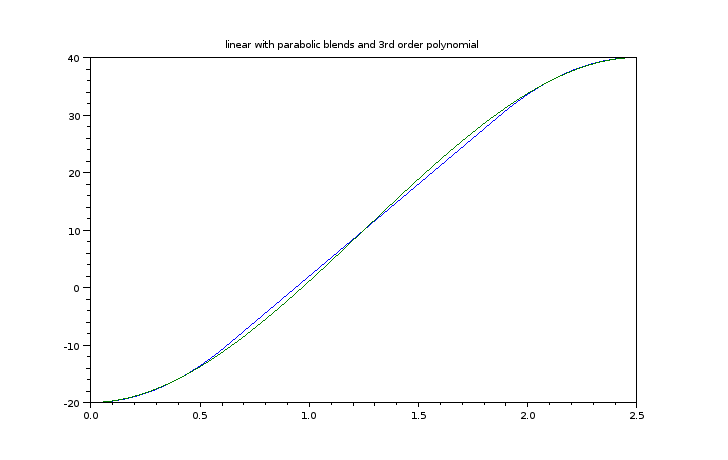
\includegraphics[width=3.5in]{trajtestscilab.png}

Note the two are very similar but not exactly the same.

\begin{verbatim}



//////////////////// Gravity Compensation Test Cases
// test case 5: gravity comp for manip of Example 3.2

clear all;
exec('tg_gravcomp.sce',-1)
 
l0 = 0.75;
l1 = 1.7;
l2 = 1.337;

al0 = -90;     al1 = 90;    al2 = 90;
a0  = 0;      a1 = l1;     a2 = l2;
d1  = l0;     d2 = 0.2;    d3 = 0;

// Pose: 
th1 = 10; th2 = 12.7; th3 = -27.6;

// coms
C11 = [0.5,0,0]';  C22 = [.2,.7,.15]';  C33 = [.4,0.1,0]';

// link masses

M(1) = 1.0;
M(2) = 1.0;
M(3) = 0.5;

// Link Transforms

T01 = link(al0, a0, d1, th1);
T12 = link(al1, a1, d2, th2);
T23 = link(al2, a2, d3, th3);

// build the T matrix vector

T = tcat(T01,T12);
T = tcat(  T,T23);

// build the COM vector

C(:,1) = C11;
C(:,2) = C22;
C(:,3) = C33;

// gravity (Planet Earth!)
g00 = [0,0,-9.8]';

// compute the gravity torques
t = jtorque(T,C,M,g00);

disp(t)

    7.2831267  
  - 1.3118838  
  - 1.8538718  
 

M(3) = 2.5;   //increase mass 3 

// compute the gravity torques again
t = jtorque(T,C,M,g00);

disp(t)

    14.501284  
  - 1.6117897  
  - 9.269359   
 
\end{verbatim}




\end{document}


%%%%** Section 5.2
\subsection{Test Cases}
